\section{Methodology}

\subsection{Research Design}
To investigate the usability, technology acceptance, and perceived cognitive workload of the proposed Jupyter dashboard extension, the study follows a quantitative, exploratory, cross-sectional evaluation design. Using standardized questionnaires, the research assesses students' initial perceptions of a learner-facing dashboard within a Jupyter-based programming environment. This evaluation serves as a necessary first step to ensure the tool is intuitive and low-burden before its long-term impact on learning outcomes can be tested.

This study focuses on answering the following research questions:
\begin{enumerate}
    \item \textbf{RQ1:} How do students evaluate the usability of the learner-facing dashboard?
    \item \textbf{RQ2:} How do students perceive the usefulness and ease of use of the dashboard?
\end{enumerate}
As the research is not intended to test causal effects, it does not employ experimental conditions such as deliberate manipulation of variables or comparisons between control and experimental groups. Accordingly, the data are collected at one point in time only, with no longitudinal measurements taken. The main purpose of this study is to evaluate usability and usefulness of the programmed learner-facing dashboard, while the results may provide a basis for further research.
Quantitative data analysis, including the calculation of descriptive statistics and Spearman rank correlations, was performed using IBM SPSS Statistics.

\subsection{Dashboard Design}

The learner-facing dashboard was designed to provide students with insights into their learning process and to support self-reflection while working in a Jupyter-based programming environment. The dashboard includes features such as visualizations of coding activity, error patterns, and progress over time. It aims to help students identify areas where they may be struggling and to encourage them to reflect on their learning strategies. The dashboard was developed as a JupyterLab extension, allowing it to seamlessly integrate with the existing workflow of students using Jupyter notebooks for programming tasks. The design process has two main components: the data collection mechanism, which captures relevant information about students' interactions with the Jupyter environment; and the data visualization component, which presents this information in an accessible and informative way.

\subsubsection{Data Collection}

The data collection mechanism is implemented using JupyterLab's extension API~\cite{jupyterlab_tutorial_2024, jupyterlab_extension_template}. From the start of the JupyterLab session, the extension monitors various events such as notebook openings, cell executions, errors, etc. Each event triggers a callback function in the backend Python code, which then stores the relevant information in a SQLite database following a predefined schema. The information collected is organized into different tables:
\begin{description}
    \item[Users] This table stores information about the users, including a personal code and their role, which could be student or teacher. Even though in our project only the student role is relevant, we have included the teacher role for potential future use. Regarding the personal code, it is used to identify users while maintaining their anonymity. This code is only used to link the data collected from the JupyterLab extension to the survey responses, allowing us to analyze the relationship between students' interactions with the dashboard and their perceptions of its usefulness.
    
    \item[Notebooks] This table contains information about the notebooks that students interact with, including the notebook title, its path and, if available, its author.
    
    \item[Notebook Sessions] This table captures the sessions of interaction with notebooks. A notebook session is defined as the period of time during which a student has a notebook open; therefore, when the active notebook changes, the previous session is closed and a new one is opened. This table registers which notebook was opened by which user, and the start and end timestamps of the session.
    
    \item[Cells] This table stores information about the cells within the notebooks, including the cell type, which can be code, markdown or raw, the cell content at the moment of its creation, the notebook it belongs to, and its Jupyter cell ID.
    
    \item[Active Cells] This table captures the active cells during a notebook session. An active cell is the cell that the user is currently interacting with. This table registers which cell was active during which notebook session, and the start and end timestamps of the active period.
    
    \item[Cell Executions] This table records the executions of code cells. for each execution, it stores the cell that was executed, the notebook session during which it was executed, the start and end timestamps of the execution, the content of the cell at the moment of execution, and the output of the execution. Regarding the errors, the number of errors and the error message are also stored in this table.
\end{description}

All the data collected and stored in the database provides plenty of possibilities for analysis and visualizations, which can help students to understand their learning process and to identify areas for improvement.


\subsubsection{Data Visualization}

The data visualization component of the dashboard is designed to present the collected information to the students in an accessible and informative way. The dashboard may be opened using the command palette as a side panel in JupyterLab, allowing students to easily access it while working on their notebooks. The dashboard includes various visualizations, which are intended to help students reflect on their learning process and to identify areas where they may need additional support or practice. A general overview of the dashboard's design and features is provided in Figure~\ref{fig:dash:general}.
\begin{figure}
    \centering
    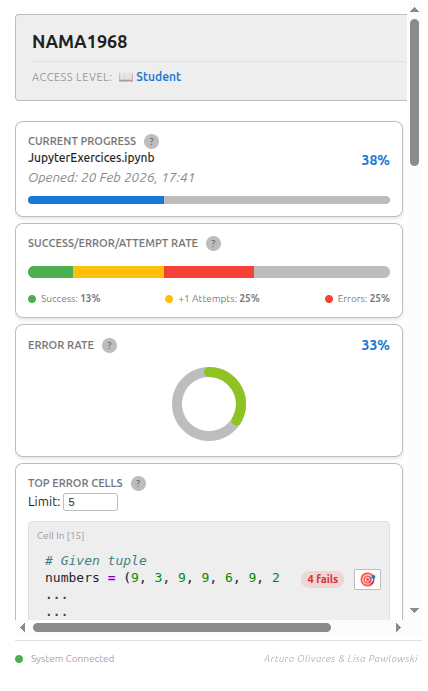
\includegraphics[scale=0.5]{img/Dashboard/general.png}
    \caption{General overview of the dashboard design.}
    \label{fig:dash:general}
    \Description{General overview of the dashboard design. The different panels of the dashboard are shown, including the user information panel, the current progress panel, the success/error/attempt rate panel, the error rate panel and the top error cells panel.}
\end{figure}
The dashboard is organized into different panels, each of which providing the students with relevant information. In addition to the visualizations, each panel includes a help button that provides a brief explanation of the information being presented and how it can be interpreted. The panels available in the dashboard are:
\begin{description}
    \item[User Information] (Figure~\ref{fig:dash:user_info}) This panel displays the user's personal code and their role.
    \begin{figure}
        \centering
        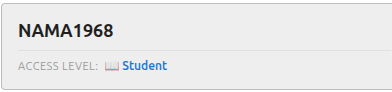
\includegraphics[scale=0.5]{img/Dashboard/user_info.png}
        \caption{User information panel.}
        \label{fig:dash:user_info}
        \Description{User information panel. The user's personal code and role are displayed.}
    \end{figure}

    \item[Current Progress] (Figure~\ref{fig:dash:current_progress}) This panel provides, apart from the title of the notebook and the opening time of the current notebook session, a visualization of the student's progress in the current notebook session. The progress is calculated as described in Equation~\eqref{eq:progress}.
    \begin{equation}\label{eq:progress}
        \text{Progress} = \frac{\text{Number of code cells with an execution without errors}}{\text{Total number of code cells}}
        \times 100\%
    \end{equation}
    \begin{figure}
        \centering
        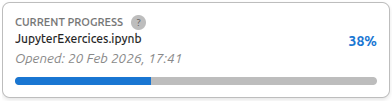
\includegraphics[scale=0.5]{img/Dashboard/current_progress.png}
        \caption{Current progress panel.}
        \label{fig:dash:current_progress}
        \Description{Current progress panel. The title of the notebook, the opening time of the current notebook session and a visualization of the student's progress in the current notebook session are displayed.}
    \end{figure}

    \item[Success/Error/Attempt Rate] (Figure~\ref{fig:dash:success_error_attempt_rate}) This panel provides a more detailed view of the student's progress. It classifies the code cells into three categories:
    \begin{itemize}
        \item Successful cells: code cells with only one execution, and that execution did not produce any errors.
        \item Attempted cells: code cells with more than one execution, having the last execution without errors.
        \item Error cells: code cells where the last execution produced an error.
    \end{itemize}
    The panel shows the rate of successful, attempted and error cells in the current notebook session, calculated as described in the Equation~\eqref{eq:rates}.
    \begin{equation}\label{eq:rates}
        \text{Rate} = \frac{\text{Number of cells in the category}}{\text{Total number of code cells}}
        \times 100\%
    \end{equation}
    \begin{figure}
        \centering
        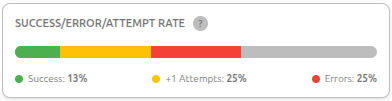
\includegraphics[scale=0.5]{img/Dashboard/success_error_attempt_rate.png}
        \caption{Success/Error/Attempt rate panel.}
        \label{fig:dash:success_error_attempt_rate}
        \Description{Success/Error/Attempt rate panel. The rate of successful, attempted and error cells in the current notebook session is displayed.}
    \end{figure}

    \item[Error Rate] (Figure~\ref{fig:dash:error_rate}) This panel focuses on the error rate in the current notebook session, calculated as described in Equation~\eqref{eq:error_rate}. It should be noted that the color used in the visualization changes according to the error rate, being green for $0\%$, red for $100\%$, and a gradient of colors in between for the values in between.
    \begin{equation}\label{eq:error_rate}
        \text{Error Rate} = \frac{\text{Number of executions with errors}}{\text{Total number of executions}}
        \times 100\%
    \end{equation}
    \begin{figure}
        \centering
        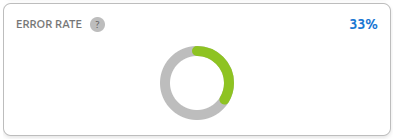
\includegraphics[scale=0.5]{img/Dashboard/error_rate.png}
        \caption{Error rate panel.}
        \label{fig:dash:error_rate}
        \Description{Error rate panel. The error rate in the current notebook session is displayed.}
    \end{figure}

    \item[Top Error Cells] (Figure~\ref{fig:dash:top_error_cells}) This panel shows the top $n$ code cells with the highest number of executions with errors in the current notebook session. The parameter $n$ can be configured by the user, allowing them to choose how many cells they want to see in this panel. The cells are ordered from the one with the highest number of executions with errors to the one with the lowest. For each cell, the panel displays the cell content of the last execution, the number of executions with errors, and a button that allows the user to jump to the cell in the notebook.
    \begin{figure}
        \centering
        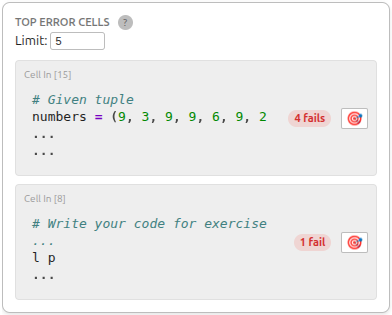
\includegraphics[scale=0.5]{img/Dashboard/top_error_cells.png}
        \caption{Top error cells panel.}
        \label{fig:dash:top_error_cells}
        \Description{Top error cells panel. The top error cells in the current notebook session are displayed.}
    \end{figure}

    \item[Top Attempt Cells] (Figure~\ref{fig:dash:top_attempt_cells}) This panel shows the top $n$ code cells with the highest number of executions in the current notebook session. For each cell, the panel displays the total number of executions.
    \begin{figure}
        \centering
        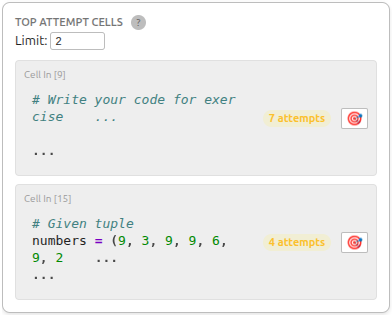
\includegraphics[scale=0.5]{img/Dashboard/top_attempt_cells.png}
        \caption{Top attempt cells panel.}
        \label{fig:dash:top_attempt_cells}
        \Description{Top attempt cells panel. The top attempt cells in the current notebook session are displayed.}
    \end{figure}

    \item[Top Time-Consuming Cells] (Figure~\ref{fig:dash:top_time_consuming_cells}) This panel shows the top $n$ code cells with the highest total execution time in the current notebook session. For each cell, the panel displays the total time that the cell has been active during the notebook session.
    \begin{figure}
        \centering
        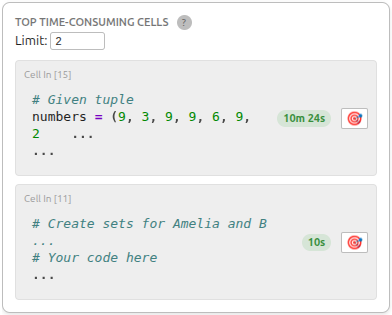
\includegraphics[scale=0.5]{img/Dashboard/top_time_consuming_cells.png}
        \caption{Top time-consuming cells panel.}
        \label{fig:dash:top_time_consuming_cells}
        \Description{Top time-consuming cells panel. The top time-consuming cells in the current notebook session are displayed.}
    \end{figure}

    \item[Top Common Error Types] (Figure~\ref{fig:dash:top_common_error_types}) This panel shows the top $n$ most common Python error types in the current notebook session, such as \texttt{IndexError}, \texttt{SyntaxError} or \texttt{NameError}. For each error type, the panel displays the number of occurrences of that error type.
    \begin{figure}
        \centering
        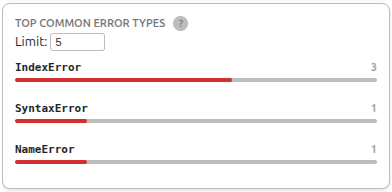
\includegraphics[scale=0.5]{img/Dashboard/top_common_error_types.png}
        \caption{Top common error types panel.}
        \label{fig:dash:top_common_error_types}
        \Description{Top common error types panel. The top common error types in the current notebook session are displayed.}
    \end{figure}

    \item[Execution Timeline] (Figure~\ref{fig:dash:execution_timeline}) This panel provides a timeline visualization of the code cell executions in the current notebook session. Each execution is represented as a point on the timeline, being the color of the point green if the execution was successful, and red if it produced an error. This visualization allows students to see the distribution of their successful and unsuccessful executions over time.
    \begin{figure}
        \centering
        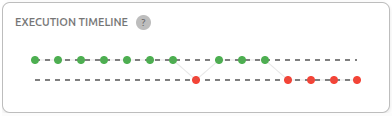
\includegraphics[scale=0.5]{img/Dashboard/execution_timeline.png}
        \caption{Execution timeline panel.}
        \label{fig:dash:execution_timeline}
        \Description{Execution timeline panel. The execution timeline in the current notebook session is displayed.}
    \end{figure}
\end{description}

\subsection{Survey Design}

The survey is designed to collect data on students' perceptions of the learner-facing dashboard in a Jupyter-based programming environment.

\subsubsection{Data Collection}

Before the data collection could start, the study was reviewed and approved by the Ethics Committee of the University of Duisburg-Essen. The ethics approval ID is 2601CMPL2910.
The data were collected via an online survey using LimeSurvey, in which participants could take part only once (see Appendix~\ref{sec:appendix_questionnaires}).
This standardized survey design ensured that all participants answered the questions in the same order in order to reduce potential confounding variables that might arise from differing procedures. In this way, a high level of replicability of the study could be ensured.

At the beginning of the study, participants were informed about the purpose of the study and the associated ethical aspects. It was made clear that participation was voluntary and that participants could withdraw from the study at any time without providing reasons or facing any consequences. Prior to starting the survey, participants were therefore required to give their informed consent. The questionnaire then began with initial questions regarding their previous experience with Jupyter Notebook and Python for comparison purposes. After that, the students began testing the Jupyter Dashboard while solving Python exercises.
Subsequently, questionnaires measuring usability and usefulness of the Jupyter Dashboard and a person's subjective mental workload by assessing six key dimensions such as mental demand, physical demand, temporal demand, performance, effort, and frustration level were administered.
This was followed by the collection of sociodemographic information, including age, gender, course of study and what semester the participants are in, in order to better describe and analyze the sample. A control question was added at the end to check whether the subjects had completed the questionnaire honestly and carefully. Finally, participants were informed about the further course of the study and thanked for their participation.

\subsubsection{Measurements}

The usability of the dashboard was assessed using the System Usability Scale (SUS)~\cite{germanupa_sus}. The SUS is a standardized and widely used instrument for evaluating the perceived usability of interactive systems. It consists of 10 items that capture users' subjective assessment of system usability, including aspects such as complexity, ease of use, and confidence in using the system. The items are rated on a 5-point Likert scale ranging from 1 (``strongly disagree'') to 5 (``strongly agree''). The scale includes five positively worded and five negatively worded items, requiring reverse coding of the negatively formulated statements prior to analysis. A sample item is: ``I thought the system was easy to use.'' The SUS score is calculated by converting item responses according to the standard scoring procedure and multiplying the sum by 2.5, resulting in a total score ranging from 0 to 100, with higher values indicating higher perceived usability. A score above 68 is commonly interpreted as indicating above-average usability. The SUS was chosen because it has demonstrated good reliability and validity across a wide range of domains and technologies with a Cronbach's Alpha $=.95$~\cite{chu2019usability}.

Perceived usefulness and acceptance of the dashboard were measured using constructs derived from the Technology Acceptance Model (TAM)~\cite{davis1989technology}. According to the model, individuals' intention to use a system is primarily determined by their perceived usefulness and perceived ease of use. Perceived usefulness refers to the extent to which a person believes that using a particular system enhances their performance, whereas perceived ease of use reflects the degree to which a person believes that using the system is free of effort. All items were rated on a 7-point Likert scale ranging from 1 (``extremely unlikely'') to 7 (``extremely likely''). Example items include statements such as ``Using the dashboard improves my learning performance'' and ``I find the dashboard easy to use.'' For each construct, mean scores were calculated by averaging the corresponding items, with higher values indicating stronger agreement. The TAM has been widely validated across technological and educational contexts and typically demonstrates good internal consistency for both dimensions with a Cronbach's Alpha $=.89$~\cite{masrom2007technology}.

Perceived workload associated with using the dashboard was assessed using the NASA Task Load Index~\cite{hart1988development}.
The NASA-TLX is a widely used multidimensional instrument for measuring subjective workload in human-computer interaction and learning environments. It captures the overall perceived task load across six dimensions: mental demand, physical demand, temporal demand, performance, effort, and frustration~\cite{hart1988development}.
